\section{Evaluation}\label{sec:eval}

In order to measure how interesting and interactive our \tube is, we developed our application to be able to take inputs from traditional input devices (\ie mouse and keyboard) and our \tube. For instance, in the balloon popping game the users will be able shoot down the balloons by clicking on the mouse and matching the color of the balloons and the mouse pointer that the user is controlling, the user will need to press some keys in the keyboard.

After describing to our participants how our \tube works, the participants tried out the applications that we have developed both with and mouse and keyboard and with \tube as the input device.

% \marginpar{
% \begin{figure}
%   \begin{center}
%   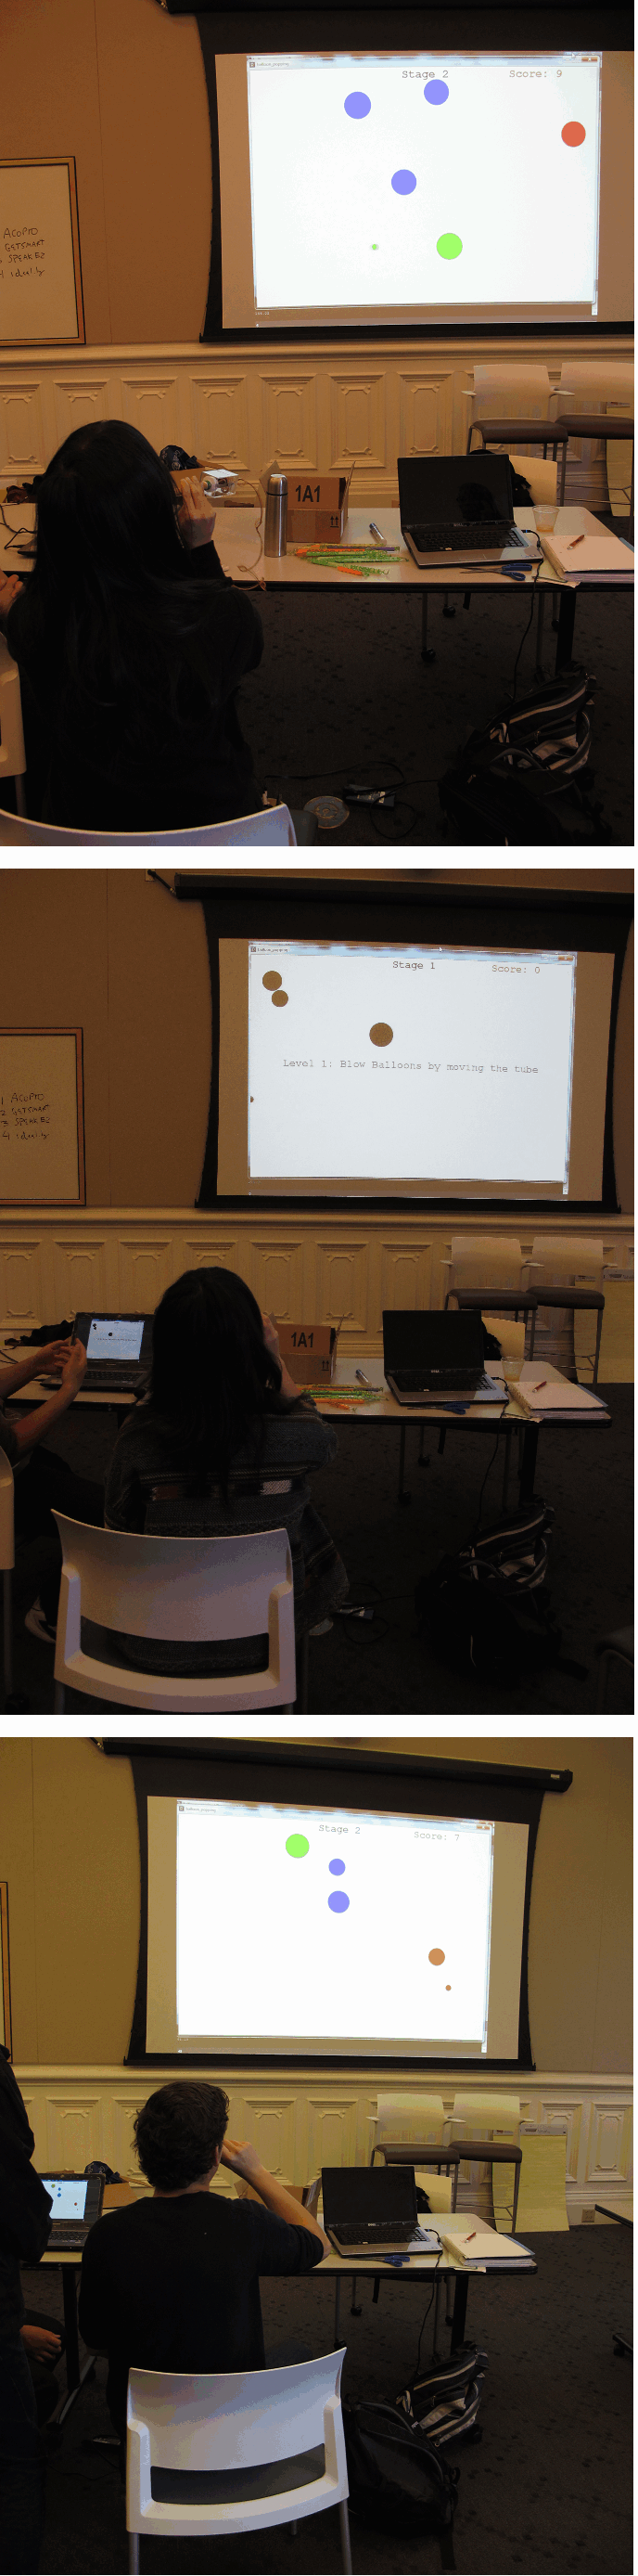
\includegraphics[width=0.7\marginparwidth]{./figs/eval.png}
%   \label{fig:eval}
%   \end{center}
% \end{figure}
% }

The first thing that our testers do when trying out the \tube was figuring how to control the small pointer on the screen. Since there is a feedback from the screen to show where the pointer is, our testers adapt to the system naturally and in no time successfully playing with \tube. Additionally, the exploding animation and the sound impact that is generated whenever the balloon is popped have really given the users a sense of satisfaction.

\begin{figure}
  \centering
  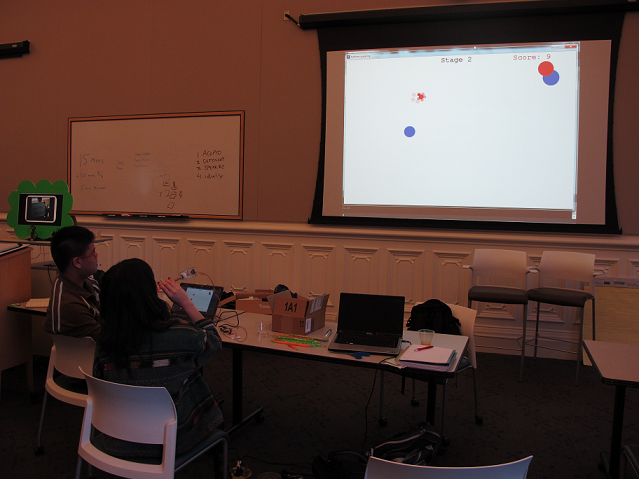
\includegraphics[width=\linewidth]{./figs/impl2.png}
  \caption{The participants trying out The \tube during a project showcase on December 7th 2011 at UC Berkeley campus.}
  \label{fig:impl2}
\end{figure}

The challenging part is when you have to match the color with the color of the balloon by rotating the tube. This is when the unique interaction with the system starts. It is not that obvious for our testers that they need to rotate the \tube in order to match its color. However, after observing that they are not able to pop the balloon without matching the colors, they start experimenting with moving the \tube in a different way and start rotating while blowing the tube. However, we may need to improve on our hardware design since some users lamented on the sensitivity of our \tube.
